% Diagram: Multi-Head Attention
\begin{figure}[htbp]
\centering
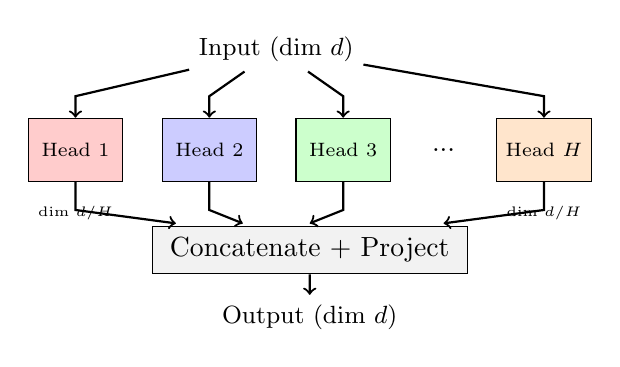
\begin{tikzpicture}[
    scale=0.85,
    head/.style={rectangle, draw, minimum width=1.2cm, minimum height=0.8cm, font=\scriptsize},
    arrow/.style={->, thick}
]
% Input
\node (input) at (0, 3) {\small Input (dim $d$)};

% Split into heads
\node[head, fill=red!20] at (-3, 1.5) (h1) {Head 1};
\node[head, fill=blue!20] at (-1, 1.5) (h2) {Head 2};
\node[head, fill=green!20] at (1, 1.5) (h3) {Head 3};
\node at (2.5, 1.5) {...};
\node[head, fill=orange!20] at (4, 1.5) (hn) {Head $H$};

% Arrows from input
\draw[arrow] (input) -- (-3, 2.3) -- (h1);
\draw[arrow] (input) -- (-1, 2.3) -- (h2);
\draw[arrow] (input) -- (1, 2.3) -- (h3);
\draw[arrow] (input) -- (4, 2.3) -- (hn);

% Concatenate
\node[rectangle, draw, minimum width=4cm, minimum height=0.6cm, fill=gray!10] at (0.5, 0) (concat) {Concatenate + Project};

% Arrows to concat
\draw[arrow] (h1) -- (-3, 0.6) -- (-1.5, 0.4);
\draw[arrow] (h2) -- (-1, 0.6) -- (-0.5, 0.4);
\draw[arrow] (h3) -- (1, 0.6) -- (0.5, 0.4);
\draw[arrow] (hn) -- (4, 0.6) -- (2.5, 0.4);

% Output
\node at (0.5, -1) (output) {\small Output (dim $d$)};
\draw[arrow] (concat) -- (output);

% Annotations
\node[below of=h1, yshift=0.2cm, font=\tiny, align=center] {dim $d/H$};
\node[below of=hn, yshift=0.2cm, font=\tiny, align=center] {dim $d/H$};

\end{tikzpicture}
\caption{Multi-head attention: input is split across $H$ heads, each processing $d/H$ dimensions independently.}
\label{fig:multi-head-attention}
\end{figure}
